\documentclass{article}
\usepackage[utf8]{inputenc}
\usepackage{amsmath}
\usepackage{graphicx}

\title{Assignment 7}
\author{Swapnil Sirsat}
\date{January 2021}

\begin{document}

\maketitle

\section*{Question}
Draw a circle of radius \textbf{3} units. Take two points
\textbf{P} and \textbf{Q} on one of its extended diameter each
at a distance of \textbf{7} units from its centre. Draw
tangents to the circle from these two points \textbf{P}
and \textbf{Q}.
\section*{Answer}
Taking the center of the circle at (0,0)
\begin{gather*}
    O = (0,0)
\end{gather*}
Taking the diameter of the circle lie on the X axis \\
the extended diameter \textbf{PQ} would be
\begin{gather*}
    P = (-7,0)\\
    Q = (7,0)
\end{gather*}
now, constructing circles with the mid point of \textbf{OP} and \textbf{OQ} as centers and  \textbf{OP} and \textbf{OQ} as diameters respectively we obtain circle R and S as coordinates
\begin{gather*}
    R = (-3.5,0)\\
    S = (3.5,0)
\end{gather*}
the intersection points of Circle \textbf{R(-3.5,0)} and \textbf{S(-3.5,0)} with \textbf{O(0,0)} would be the points of contact of tangents through P and Q respectively
\\this point would be as
\\For tangents through P, solving the equations  
\begin{gather}
    x^{2} + y^{2} = 9\\
    (x+3.5)^{2} + y^{2} = (3.5)^{2}
\end{gather}
we would obtain the point of contact for the tangents\\
similarly for tangents through Q, solving the equation (1) and
\begin{gather}
    (x-3.5)^{2} + y^{2} = (3.5)^{2}
\end{gather}
we would obtain the point of contact for the tangents\\
equation (2) can be rewritten as 
\begin{gather}
   x^{2} + (3.5)^{2} + 2\times(3.5)\times x + y^{2} = (3.5)^2\\
   \implies  x^{2} + y^{2} + (3.5)^{2} + 2\times(3.5)\times x = (3.5)^2
\end{gather}
and equation (3) can be rewritten as 
\begin{gather}
    x^{2} + (3.5)^{2} - 2\times(3.5)\times x + y^{2} = (3.5)^2\\
    \implies  x^{2} + y^{2} + (3.5)^{2} - 2\times(3.5)\times x = (3.5)^2
\end{gather}
substituting equation (1) in (5) we get
\begin{gather*}
    9 +  (3.5)^{2} + 2\times(3.5)\times x = (3.5)^2\\
    \implies 9 + 7x = 0\\
    \implies x = \frac{-9}{7} = -1.286\\
\end{gather*}
substituting value of x in equation (1)
\begin{gather*}
    (\frac{-9}{7})^{2}+y^{2} = 9\\
    \implies y = \sqrt{9-(\frac{-9}{7})^{2}}\\
    \implies y = \pm 2.710
\end{gather*}
Similarly substituting equation (1) in (7) we get x = $\frac{9}{7}$ = -1.286
\\and substituting this in equation 1 we get
\begin{gather*}
     y = \pm 2.71 
\end{gather*}
therefore the tangents from P would make contact with Circle O at
\begin{gather*}
    T_1(-1.286,2.710)\\
    T_2(-1.286,-2.710)
\end{gather*}
and tangents from Q would make contact at 
\begin{gather*}
    T_3(1.286,2.710)\\
    T_4(1.286,-2.710)
\end{gather*}
\\ joining this points we would obtain the asked tangents on circle O.
\newpage
below is the constructed figure.
\begin{figure}[h!]
    \centering
    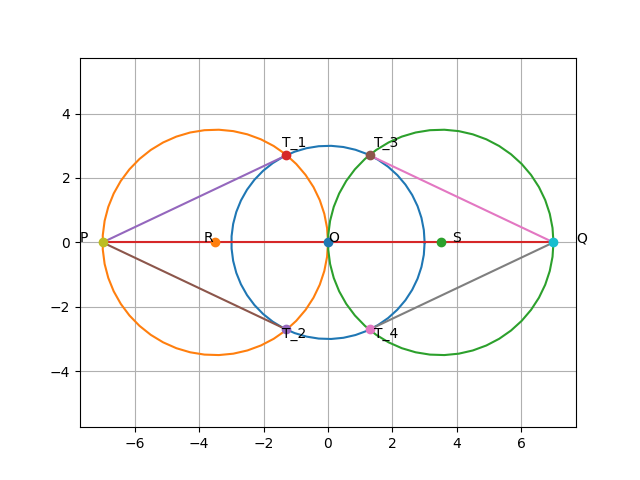
\includegraphics{Figure_1.png}
    \caption{Python output}
    \label{fig:my_label}
\end{figure}

\end{document}
